\documentclass[11pt]{article}
%\usepackage[framemethod=tikz]{mdframed}
\usepackage{tcolorbox}
\usepackage{titling}
%\usepackage{figure}
\usepackage[os=win]{menukeys}
\newcommand{\numpy}{{\tt numpy}}    % tt font for numpy

\topmargin -.5in
\textheight 9in
\oddsidemargin -.25in
\evensidemargin -.25in
\textwidth 7in

\pretitle{%
  \begin{center}
  \LARGE
  
\includegraphics[width=15cm]{../images/logo.png}\\[\bigskipamount]
}
\posttitle{\end{center}}

\begin{document}

% ========== Edit your name here
\author{Dr. Neil Eliot / Dr. Alun Moon}
\title{KF5004\\------\\Workshop 7\\------\\Setting up \texttt{subdomains}\\------}
\date{September 2019}
\maketitle

\newpage

% \begin{center}
%     \noindent\rule{8cm}{0.4pt}
% \end{center}

% ========== Introduction

\noindent\textbf{Learning Outcomes:}
\begin{itemize}
    \item Understand what a \texttt{subdomain} is.
    \item Configure \texttt{subdomain}s:
        \begin{itemize}
            \item Full delegation.
            \item Pseudo/Virtual delegation.
        \end{itemize}
\end{itemize}

% \begin{center}
% \noindent\rule{8cm}{0.4pt}
% \end{center}

\begin{tcolorbox}[title={\textbf{Important:}}]
    Before you begin, ensure the lab. \texttt{PC} you are using is connected to the off campus lab infrastructure and the machine receives an \texttt{IP} address from the lab. \texttt{DHCP} Server.
\end{tcolorbox}
\newpage

\noindent\textbf{The Exercise}\\
\begin{tcolorbox}[colback=blue!20]
    \noindent\textbf{From the commands and processes defined in the lecture carry out the following:}
\end{tcolorbox}

% ========== Begin answering questions here

\begin{tcolorbox}[title={\textbf{NOTE:}}]
    In this workshop you should use your virtual \texttt{Ubuntu Desktop} that you create in the first workshop. \textbf{Please do not alter the base machines in the laboratory}.
\end{tcolorbox}

\begin{enumerate}
    \item Create a \texttt{DNS} architecture consisting of 3 servers as illustrated in Fig~\ref{dnsarch1} as \texttt{NS1, NS3 \& NS4}. (You will create \texttt{NS2} later in the workshop).
        \begin{tcolorbox}[title={\textbf{NOTE:}}]
            \noindent Don't forget. These are servers and \textbf{SHOULD} have static addresses. Use \texttt{IP} addresses from your provided range.
        \end{tcolorbox}
    \begin{itemize}
            \item 1 \texttt{Primary} server (\texttt{NS1}).
            \item 2 \texttt{Secondary} servers (\texttt{NS3 \& NS4}).
        \end{itemize}
        \begin{figure}[ht]
            \begin{center}
              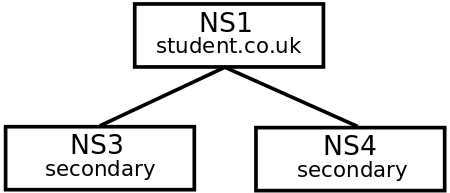
\includegraphics[width=.35\linewidth]{subdomainWS1.png}  
              \caption{Single \texttt{domain} Architecture}
              \label{dnsarch1}
            \end{center}
        \end{figure}
    \item Add a zone of \texttt{student.co.uk} and a reverse zone consisting of the following records:
        \begin{tcolorbox}[title={\textbf{NOTE:}}]
            \noindent Only implement \texttt{www} and \texttt{mail} in the \texttt{rDNS}.\\
            \noindent All \texttt{IP} addresses are in the range \texttt{192.168.0.0/16} (subnet mask \texttt{255.255.0.0}).
        \end{tcolorbox}
        \begin{itemize}
            \item \texttt{192.168.100.2} $\Leftrightarrow$ \texttt{www2.student.co.uk}
            \item \texttt{192.168.100.2} $\Leftrightarrow$ \texttt{www.student.co.uk}
            \item \texttt{<your client IP>} $\Leftrightarrow$ \texttt{me.student.co.uk}
            \item \texttt{192.168.100.21} $\Leftrightarrow$ \texttt{server.student.co.uk}
            \item \texttt{192.168.100.2} $\Leftrightarrow$ \texttt{mail.student.co.uk}
            \item \texttt{192.168.100.254} $\Leftrightarrow$ \texttt{gateway.student.co.uk}
        \end{itemize}
    \item Test your \texttt{zone} file has no errors.
    \item \label{itm:queries} Test the following queries:
        \begin{itemize}
            \item \texttt{192.168.100.2}
            \item \texttt{www.student.co.uk}
        \end{itemize}
    \item Create a further \texttt{DNS} server (\texttt{NS2}). (This will be the \texttt{Primary server} for the \texttt{subdomains}).
        \begin{figure}[ht]
            \begin{center}
              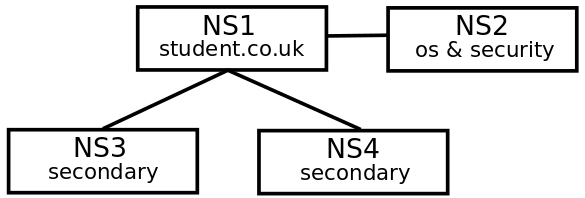
\includegraphics[width=.5\linewidth]{subdomainWS2.png}  
                \caption{\texttt{subdomain} Architecture}
                \label{dnsarch2}
            \end{center}
        \end{figure}
    \begin{itemize}
            \item Statically address the new server and install \texttt{bind9} and \texttt{dnsutils}.
            \item Add two \texttt{subdomains}.
                \begin{itemize}
                    \item \texttt{os.student.co.uk}
                    \item \texttt{security.student.co.uk}
                \end{itemize}
            \item Add the following \texttt{hostnames} to both \texttt{subdomains} with some random \texttt{IP} addresses.
                \begin{itemize}
                    \item \texttt{www}
                    \item \texttt{ftp}
                    \item \texttt{server1}
                    \item \texttt{server2}
                \end{itemize}
            \item Add \texttt{rDNS} records for the \texttt{www} and \texttt{ftp} servers.
            \item Test that all the new entries resolve correctly.
            \item Link the \texttt{subdomains} to the \texttt{Primary server} (HINT: as \texttt{slaves})
            \item Prevent any machines from querying the new server. 
        \end{itemize}
    \item Update the \texttt{Primary server} (\texttt{NS1}) to implement the \texttt{subdomains} defined above using a single \texttt{zone} file.
    \item Update the \texttt{Primary server} (\texttt{NS1}) to implement the \texttt{subdomains} defined above using one additional (\texttt{include}) \texttt{zone} file.
\end{enumerate}    
END
\end{document}